% Created 2020-05-06 mié 14:05
% Intended LaTeX compiler: pdflatex
\documentclass[a4paper, 12pt]{article}
\usepackage[utf8]{inputenc}
\usepackage[T1]{fontenc}
\usepackage{graphicx}
\usepackage{grffile}
\usepackage{longtable}
\usepackage{wrapfig}
\usepackage{rotating}
\usepackage[normalem]{ulem}
\usepackage{amsmath}
\usepackage{textcomp}
\usepackage{amssymb}
\usepackage{capt-of}
\usepackage{hyperref}
\usepackage{float, amsfonts, commath, mathtools, proba}
\author{Tabaré Pérez}
\date{\today}
\title{Lecture 15 - 9: Gaussian Generative models}
\hypersetup{
 pdfauthor={Tabaré Pérez},
 pdftitle={Lecture 15 - 9: Gaussian Generative models},
 pdfkeywords={},
 pdfsubject={},
 pdfcreator={Emacs 26.3 (Org mode 9.3.6)}, 
 pdflang={English}}
\begin{document}

\maketitle
So now we finish talking about multinomials. And again, just to recap, when we
talk about multinomials, I described to you how to estimate \(\theta\)s. And we
discussed how we can use these multinomials to make predictions. Now, we're
going to switch gears and look at a different example. We will start talking
about \textbf{Gaussians}. So before we're talking about the words. Now we are going to
go to vectors in \(\mathbb{R}^d\) and find distribution that is a very natural
fit for describing this data.

So now, we will start talking about Gaussians. And it is appropriate to use
Gaussians when we are looking at vectors in \(\mathbb{R}^d\):

\begin{equation}
x \in \mathbb{R}^d
\end{equation}

And again, \(d\) is the dimensionality of the space, and Gaussian is maybe the
most of the vanilla distributions where we are looking at a cloud of points:

\begin{figure}[H]
\centering
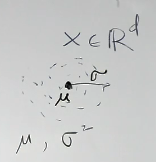
\includegraphics[width=0.5\textwidth]{./pic/u04-08-fig-01.png}
\caption{\label{fig:org5045666}Cloud of points}
\end{figure}

And the way we are going to describe these points is by two parameters. The
first parameter will be kind of where is the center of this cloud and we would
call the center is the mean \(\mu\).

And then we will also have another parameter, which is called \(\sigma^2\),
which would look at how dispersed is this cloud. Is it really tight and very
close to the center or the points can be dispersed?

Now, you can be thinking to yourself, maybe points in my particular examples are
not really nicely described at the sphere. Maybe there are actually multiple
clouds. But in this case, we are going to make an assumption that the only way
we can describe it, if we decided to use Gaussians, is actually to assume that
there is some mean for all these different clouds and there is a certain
\(\sigma^2\) that will tell you how dispersed they are. And this is actually an
important modeling point related to generative models.

You're always making assumptions. And this model that you are selecting when you
have multiple choices, you need to decide which class of models is appropriate
to your data.

So in this particular case, again, if there are even many more clouds, for now,
we will make an assumption that we will characterize them by these two
parameters.

And typically, when people think about Gaussians, in their head, they're
thinking about this sphere and again, the center here would be \(\mu\) and the
radius of this sphere would be the \(\sigma\). And farther away you go from this
\(\mu\), the lower is the likelihood that the point was generated by this
Gaussian.

And it doesn't matter to which direction do you go. So the meaning of \(\mu\)
would be just an average of all these points and \(\sigma^2\) is just the square
of the average distance of \(x\)s from the \(\mu\).

So now, we kind of discussed about what this model
is, roughly speaking, captures and we need to write the probabilities
to talk about the parameters of this probability distribution.

And as we can see here, there are just two of them. So we can write for any
point \(x\) given the parameters \(\mu\) and \(\sigma^2\), we can write the
likelihood of \(x\) to be generated by these Gaussians. So in this case, it's
going to be:

\begin{equation}
\prob(x|\mu, \sigma^2) = \frac{1}{(2\pi\sigma^2)^{\frac{d}{2}}}e^\left( {-\frac{1}{2\sigma^2} \norm{x-\mu}^2} \right)
\end{equation}

So this is just the normalization constant. And you can see the \(d\) is the
space dimension.

So this is the likelihood of a particular point being generated by the Gaussian.

And you can see that if we select different \(\mu\)s and different \(\sigma\)s,
the same point may get different likelihoods.
\end{document}